\documentclass{sigchi}

% Use this command to override the default ACM copyright statement (e.g. for preprints).
% Consult the conference website for the camera-ready copyright statement.


\toappear{
Copyright is held by the owner/author(s). Publication rights licensed to ACM.\\
{\emph{L@S'14}}, March 4--5, 2014, Atlanta, GA. \\
ACM 978-1-4503-2669-8/14/03 \\
((DOI HERE))
}

% Arabic page numbers for submission.
% Remove this line to eliminate page numbers for the camera ready copy
%\pagenumbering{arabic}


% Load basic packages
\usepackage{balance} % to better equalize the last page
\usepackage{graphics} % for EPS, load graphicx instead
\usepackage{times} % comment if you want LaTeX's default font
\usepackage{url} % llt: nicely formatted URLs
\usepackage{tabularx}

% llt: Define a global style for URLs, rather that the default one
\makeatletter
\def\url@leostyle{%
\@ifundefined{selectfont}{\def\UrlFont{\sf}}{\def\UrlFont{\small\bf\ttfamily}}}
\makeatother
\urlstyle{leo}


% To make various LaTeX processors do the right thing with page size.
\def\pprw{8.5in}
\def\pprh{11in}
\special{papersize=\pprw,\pprh}
\setlength{\paperwidth}{\pprw}
\setlength{\paperheight}{\pprh}
\setlength{\pdfpagewidth}{\pprw}
\setlength{\pdfpageheight}{\pprh}

% Make sure hyperref comes last of your loaded packages,
% to give it a fighting chance of not being over-written,
% since its job is to redefine many LaTeX commands.
\usepackage[pdftex]{hyperref}
\hypersetup{
pdftitle={L@S 2014 Work-in-Progress Format},
pdfauthor={LaTeX},
pdfkeywords={SIGCHI, proceedings, archival format},
bookmarksnumbered,
pdfstartview={FitH},
colorlinks,
citecolor=black,
filecolor=black,
linkcolor=black,
urlcolor=black,
breaklinks=true,
}

% create a shortcut to typeset table headings
\newcommand\tabhead[1]{\small\textbf{#1}}


% End of preamble. Here it comes the document.
\begin{document}

\title{Learner-Sourcing in an Engineering Class at Scale}

\numberofauthors{3}
\author{
\alignauthor Elena L. Glassman\\
\affaddr{MIT CSAIL}\\
\email{elg@mit.edu}
\alignauthor Chris Terman\\
\affaddr{MIT CSAIL}\\
\email{cjt@mit.edu}
\alignauthor Robert C. Miller\\
\affaddr{MIT CSAIL}\\
\email{rcm@mit.edu}
}

\maketitle

\begin{abstract}
Teaching computer architecture as a hands-on engineering course to approximately 250 MIT students per semester requires a large, dedicated teaching staff. This spring, a shortened version of the course will be deployed on edX to a potentially far larger cohort of students, without additional teaching staff. To better support students, we have deployed developmental versions of three learner-sourcing systems to as many as 500 students. In this work, learner-sourcing refers to crowd-sourcing within the community of students enrolled in a course. 

Our three systems have distinct objectives: (1) learner-source hints for debugging, (2) learner-source hints for optimization, and (3) prompt students to reflect on other students' solutions. These systems harvest and organize students' collective knowledge about designing and debugging solutions to assignments. The key design principle is that students write hints immediately after completing a task or fixing a bug. Later, other students can use these hints to help guide them to a correct solution or better design. We plan to deploy and study the next iteration of these systems on edX this Spring.
\end{abstract}

\keywords{
        engineering education; crowd-sourcing; learner-sourcing
}

\category{H.5.m.}{Information Interfaces and Presentation (e.g., HCI)}{Miscellaneous}


\section{Introduction}

One-on-one tutoring has been established as a costly gold standard in education \cite{Bloom}. Engineering education is no exception. By opening up the virtual classroom to thousands of students, MOOCs make the teacher-to-student ratio drastically lower. Teaching staff become even more distant from students' solutions because they can no longer walk around the lab or classroom interacting with students one-on-one to get a sense of common success and failure modes. They also suffer from the ``curse of knowledge,'' which is the difficulty experienced by experts when trying to see some concept or artifact from the perspective of a novice \cite{curse}.

We are developing systems which harvest and organize students' collective knowledge about designing and debugging solutions to assignments. Students themselves are each becoming experts on their own bugs and solutions. The key design principle is that students write hints immediately after completing a task or fixing a bug. Later, other students can use these hints to help guide them to a correct solution or better design. While students do not have the pedagogical content knowledge to necessarily generate the optimal explanations, they also do not suffer from the curse of knowledge. These systems relieve some of the pressure on the relatively small teaching staff, and give students the valuable educational experiences of reflection and generating explanations \cite{selfexplanation}. 
%\begin{figure}[!h]
%\centering
%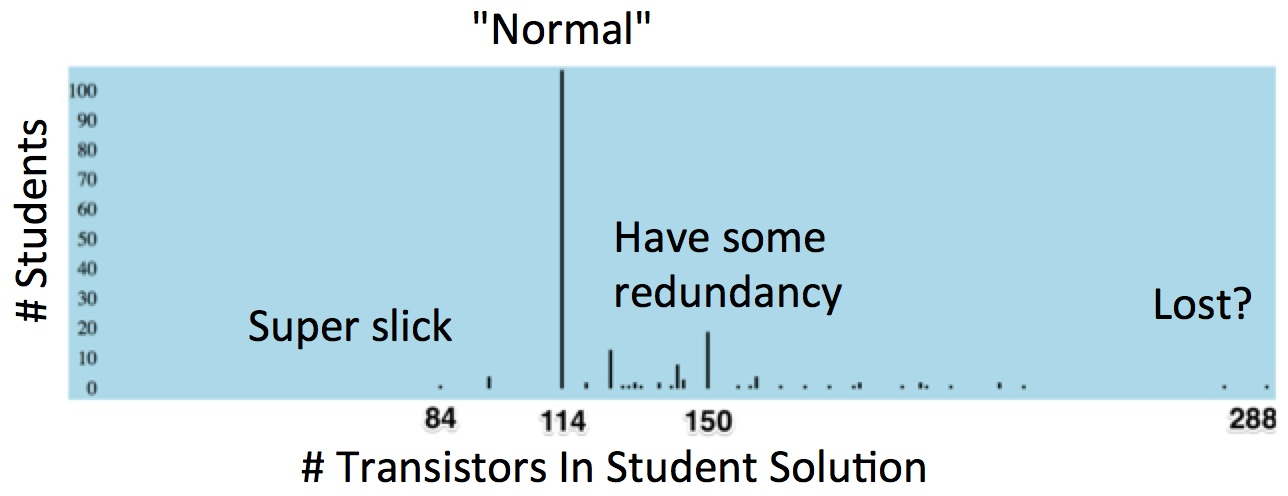
\includegraphics[width=0.9\columnwidth]{distributionOfTransistors.jpg}
%\caption{Distribution of the students' correct solutions (Full Adders), as a function of the %number of trasistors.}
%\label{fig:figure1}
%\end{figure}

We present on-going case-studies of three systems deployed in an undergraduate computer architecture course at MIT. Around two hundred and fifty students enroll each semester. To pass, students must each build an entire simulated processor out of logic gates. The three deployed systems have distinct objectives: (1) learner-source hints for debugging, (2) learner-source hints for optimization, and (3) prompt students to reflect on other students' solutions. In this work, learner-sourcing refers to crowd-sourcing within the community of students enrolled in a course.

These systems have already been deployed at scale to as many as five hundred students over multiple semesters. Our residential case-studies prepare us to design, deploy, and study the next iteration of these systems on edX this Spring. Throughout the process, we continue to develop design principles that can guide future learner-sourcing systems for engineering classes.

\section{Related Work}

In order to generate hints for others, students must reflect on their bug, solution, or optimization, and then communicate it to others. We review some relevant literature at the intersection of learning theory and engineering education.

\subsection{Reflection}
Reflection and confusion are both treated at length in learning theory literature. Piaget theorized that cognitive disequilibrium, experienced as confusion, could trigger learning: the creation or restructuring of knowledge schema \cite{disequilibrium}. However, D'Mello et al. point out that, for this learning to take place, it is important for confusion to be both appropriately injected and resolved \cite{productiveconfusion}. Dewey theorized that reflection is a critical method for triggering that transformation from conflict and doubt into clarity and coherence \cite{dewey1933}. Turning that reflection into a self-explanation also improves understanding \cite{selfexplanation}.

Given the established value of reflection, Turns et al. \cite{asee} argue that the absence of reflection in traditional engineering education scholarship is a significant gap. Professor Susan Ambrose, Northeastern's Vice Provost for Teaching and Learning has called on engineering curriculum designers to incorporate reflection \cite{ambrose}. In this work, we aim to design scalable automated opportunities for students to reflect.
\subsection{Peer Instruction and Assessment}
While reflection is valuable in its own right, it is also a building block of larger frameworks, like Peer Instruction \cite{mazur} and Peer Assessment \cite{peerassessment}. Peer instruction requires students to form educated guesses, and then discuss and reflect on their choices with peers. Peer Assessment replaces peer discussion with peer evaluation. For example, in Peer Assessment Learning Sessions \cite{pals}, students assessed each other's written calculations and sketches in numerical problem solving courses, i.e., Hydraulic Engineering and Reinforced Concrete Design. 

Reflecting on a peer's conceptual development or alternative solution may bring about cognitive conflict that prompts re-evaluation of the student's own beliefs and understanding \cite{kavanagh}. We aim to trigger productive cognitive conflict that students can attempt to resolve through written reflection.
\subsection{Generating Hints for Students}
With a mixture of automation and human input, helpful hints have been delivered students in multiple problem domains. Some of these domains can be solved by students taking one of a family of sequential steps toward the final correct answer, such as logic proofs \cite{barnes} and physics problems \cite{gertner}. Other domains are less constrained, e.g., introductory programming assignments \cite{autograder}. Finally, some domains, such as general software development, are complex enough that hints are based on errors and local information about a student's work, rather than a global understanding of that students' work \cite{helpmeout}. Our students' processors are complex enough that they fall into this third, most complex problem domain.

Hartmann et al.'s HelpMeOut \cite{helpmeout} system handles arbitrarily complex Java code by tracking and storing the changes programmers make when fixing a compilation error or runtime exception. Users, presumably students and teachers, can write helpful messages to accompany these automatically extracted bug fixes. Like HelpMeOut for hardware design, one of our systems also asks students to generate hints for peers struggling with the same bug and indexes those hints according to their associated verification failure. Another system we have deployed allows students to learner-source design optimizations, which are larger transitions from one working solution to another.

\section{Debugging: crowd-sourcing hints from learners}                                                
In our course, students design entire simulated processors composed of logic gates. These processors, expressed as pages' worth of an in-­house declarative hardware description language, can be challenging to debug even with the one­-on-­one help of seasoned teaching staff. In fact, students who have recently resolved a particular bug can be in a better position than available staff members to help a fellow student with the same bug. 

Bugs are revealed by voltage verification failures. A testbed monitors a set of simulated wires within the student's processor during execution of a staff-provided sequence of instructions. During each simulation, the testbed reports the first wire that fails verification and the time of that failure. There are hundreds of possible unique verification failures, some more common than others. The course has a Piazza forum, but the generic forum structure made it awkward and time-consuming to search for other students' questions about resolving particular verification failures.  %Yet reporting only the earliest verification failure restricts the number of distinct bugs responsible for a particular verification failure. 

\begin{figure*}
\centering
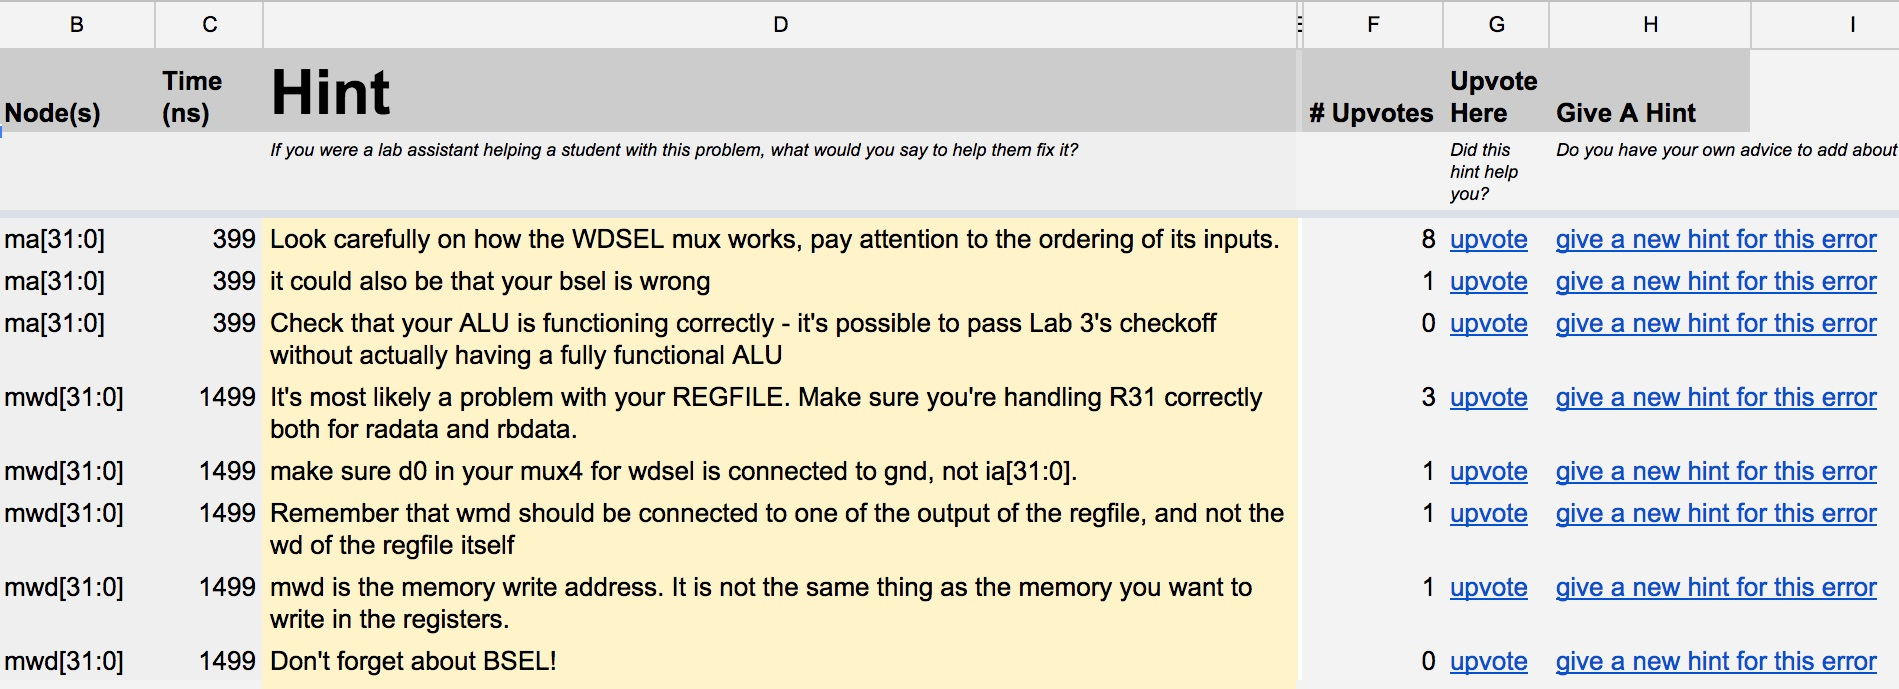
\includegraphics[width=0.75\textwidth]{DearBeta.jpg}
\caption{{\it Dear Beta} serves as a central repository of debugging advice for and by students, indexed by verification failures. For example, there are three separate crowd-sourced hints for the first verification failure ($ma[31:0], 399ns$), ordered from greatest to least upvotes. The left two columns, wire name and time, uniquely characterize the verification failure. The central pale yellow column is for the hint. The right-most three columns display the number of upvotes, a link that will add an upvote to the hint, and a link to add a different hint for the same verification error. {\it Dear Beta} is implemented with Google Spreadsheets, Forms, and Apps Scripts.}
\label{fig:figure3}
\end{figure*}

We built {\it Dear Beta}, a system that serves as a central repository of debugging advice for and by students, indexed according to verification failures. The processor in this class is called the Beta, and the system's name comes from the fact that it looks like a spreadsheet with an advice column, as shown in Figure \ref{fig:figure3}. As soon as a student resolves a bug that was causing a particular verification failure, they can post an explanation of their bug on Dear Beta along with the verification failure it caused. Providing the bug-resolving explanation is pedagogically useful, and students struggling with a particular verification failure can easily look up advice for their particular failure, if another student or staff member has added a hint. Students can upvote hints they found helpful. 

A particular verification failure may be caused by one of several possible bugs. As the number of students and/or cumulative semesters becomes sufficiently large, crowd-sourcing students' own bug-fixes may generate hints about all the possible causes of a particular verification failure. 

System usage statistics, interviews with teaching staff, and anecdotal evidence, including a student's unprompted class forum thank you note, suggest that many students find the system to be a consistently helpful tool. As one teaching assistant said, ``Whenever I came to help a student, I first asked them if they'd checked Dear Beta.'' 

We hope to create a Meteor or Django-backed version of Dear Beta for both the residential and potentially much larger online cohort of students who take the course this Spring. We anticipate that students can cover a larger fraction of verification failures with hints that are just as helpful as the original staff-provided debugging hints.


\section{Optimization: crowd-sourcing hints and results from learners}

As a final exercise in our residential course, students optimize their own processors for additional points, which are a function of the processor's size and speed. Students also get a long list of optimization hints written by staff, which students consult when choosing optimizations to implement. Students can take hours to act on a single optimization hint. Some students hear stories of the form, ``I tried {\it x} and got {\it y} points!'' One student heard that two classmates got significantly different outcomes from implementing the same two optimizations in opposite orders. This does not make sense, technically, but these kinds of optimization tales are all students have had to go on. 

We deployed a system for learner-sourcing optimization hints and results, with the aim of giving students more transparency and assistance. Rather than indexing hints based on verification failures, we indexed hints based on whether they were intended to reduce their processor's size, increase its speed, or both. We also gave students the option of submitting the magnitude of the speed and size improvement they got from acting on a hint, so that future students could gauge which optimization hints were most beneficial on average. 

This system was not as successful as Dear Beta. We are still diagnosing why it failed. For example, it did not collect hints about verification failures created {\it during} the optimization process, which were common. We are, however, confident that students are ultimately capable of generating high quality processor optimization hints, based on results shown in the next section on reflection and comparison.

\section{Reflection: Prompted Reflections on Other Students' Solutions}

In our course, one of the early digital design assignments students complete is the construction of a Full Adder. A Full Adder adds two bits of information, plus an optional `carry-in' bit, to produce a `sum' bit and `carry out' bit. Two possible solutions are shown in Figure \ref{fig:figure2}. Since the assignment only requires a working Full Adder circuit and there is no pressure to optimize their solution, students create a variety of solutions that fit the behavior specification. Some are bloated, and some make use of one or more `tricks' to use as few transistors as possible. In this scenario, fewer transistors translates to better performance.

\begin{figure}[!h]
\centering
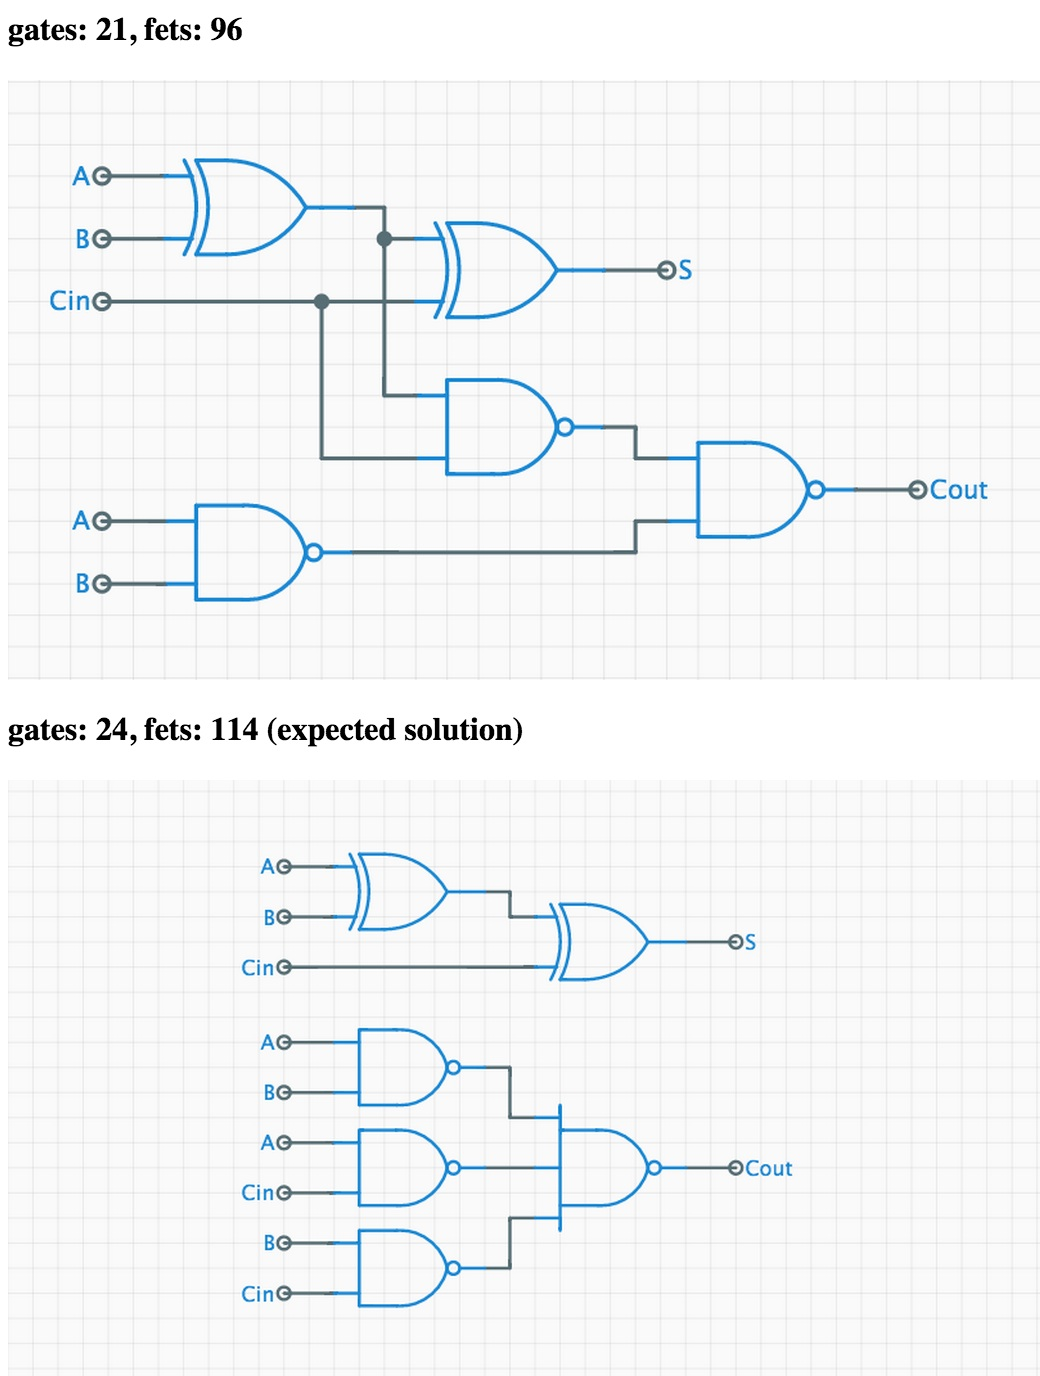
\includegraphics[width=1.0\columnwidth]{solutionComparison.jpg}
\caption{Two correct student solutions (Full Adders), composed of different numbers and arrangements of XOR and NAND gates. The more optimal solution has only 21 gates and 96 transistors (FETs) while the less optimal solution has 24 gates and 114 transistors.}
\label{fig:figure2}
\end{figure}

Through exploration of hundreds of previous students' solutions, we found that alternative correct solutions are nearly completely distinguishable by the number of transistors they contain. We picked a set of representative student solutions and rendered them graphically, rather than as raw student code. Each student was asked to compare their own solution to (1) a worse solution in the representative set and (2) to the best solution in the representative set. Figure \ref{fig:figure2} illustrates one possible pair of alternative solutions.

Students were asked to give a hint to future students about how to improve the poorer solution in each pairing. When the student's own solution is the better solution in the pair, then the student can diagnose and describe, as a hint, what the poorer solution's creator had conceptually missed. For example, {\it Remember DeMorgan's Law: you could replace the `OR' of `ANDs' with a `NAND' of `NANDs.'} When the students' own solution is the poorer solution in the pair, then they are challenged to understand how the better solution uses fewer transistors to achieve the same functionality, and then explain that to the future student that did not yet have that insight. 

\begin{table}
\begin{tabularx}{\columnwidth}{ |X| }
\hline
{\bf Learner-sourced Advice} \\
    \hline
    ``Do not try to be too clever with $C_{out}$---design your schematic as the expression is written. This way you will achieve the [standard] schematic.'' \\ \hline
    ``Keep in mind that although expressions like XOR and OR are not equivalent in isolation, when combined in a larger expression, they may serve the same purpose. Because you've already found the XOR of A and B for example, you can then use that as the OR of A and B when you know A AND B will be ANDed with A XOR B later on.'' \\ \hline
``Mutate the boolean function for $C_{out}$ such that all OR and AND operations are being NOT'ed. This allows you to design a circuit using only naturally inverting CMOS gates.'' \\ \hline 
``I would ask: is there a way for you to use some intermediate node in one circuit to bypass a CMOS gate in the other, leading to a reduction of used mosfets?'' \\ \hline
    \end{tabularx}
\caption{Examples of learner-sourced advice for optimizing fellow students' Full Adders.}
\label{tab}
\end{table}


This reflection and explanation process is pedagogically valuable on its own. In addition, students' explanations give a rich window into their understanding, while serving as strikingly cogent potential advice to future students. Table \ref{tab} shows examples of student-generated hints collected during our deployment. The online version of this course may afford us the opportunity to deliver these optimization hints back to students, when they complete a new, online-only adder optimization lab.

\section{Conclusions and Future Work}

This work in progress is the accumulation of several semesters of system development and deployment in a large undergraduate engineering course. We have found that students can write high quality optimization advice for simple digital circuits when their solution is paired with a solution that is different from theirs. We have also found that crowdsourcing students' debugging hints, indexed according to the verification failures they are associated with, is an effective way to help students help each other. We are preparing to deploy the next iteration of these systems on edX this Spring, while we actively consider how best to measure their impact on the student learning experience.

\section{Acknowledgments}

We appreciate the support of the NSF Graduate Research Fellowship, Quanta Computer, and the Amar Bose Teaching Fellowship for funding this work.

% Balancing columns in a ref list is a bit of a pain because you
% either use a hack like flushend or balance, or manually insert
% a column break. http://www.tex.ac.uk/cgi-bin/texfaq2html?label=balance
% multicols doesn't work because we're already in two-column mode,
% and flushend isn't awesome, so I choose balance. See this
% for more info: http://cs.brown.edu/system/software/latex/doc/balance.pdf
%
% Note that in a perfect world balance wants to be in the first
% column of the last page.
%
% If balance doesn't work for you, you can remove that and
% hard-code a column break into the bbl file right before you
% submit:
%
% http://stackoverflow.com/questions/2149854/how-to-manually-equalize-columns-
% in-an-ieee-paper-if-using-bibtex
%
% Or, just remove \balance and give up on balancing the last page.
%
\balance


% REFERENCES FORMAT
% References must be the same font size as other body text.

\bibliographystyle{acm-sigchi}
\bibliography{learnersourcing}
\end{document}


Scraps:

A TA will never had done it the length of time as the lecturer whose taught the course, who understands the relative frequencies and value of design decisions that students make while working on engineering challenges. Furthermore, while the TA is expected to solve the lab before coming in to help the students, they can only be expected to solve it one way, of all the potential ways students choose.

<solution: crowd-sourcing with incentives and guiding constraints> The collective activity of large classes can map out Students can become the local experts on what they implemented, which is both valuable pedagogically and from the perspective of scaling classes up without always having the staff to support them.

like describing an arithmetic logic unit in a hardware description language. 
Great professors may complete the assignment themselves in multiple ways, anticipating the approaches students might take. They may have deep pedagogical content knowledge. 
They have seen a multitude of bugs and designs, though occasionally students surprise them with something new.


\section{Page Size and Columns}

On each page your material (not including the page number) should fit
within a rectangle of 18 x 23.5 cm (7 x 9.25 in.), centered on a US
letter page, beginning 1.9 cm (.75 in.) from the top of the page, with
a .85 cm (.33 in.) space between two 8.4 cm (3.3 in.) columns. Right
margins should be justified, not ragged. Beware, especially when using
this template on a Macintosh, Word can change these dimensions in
unexpected ways. Please be sure that your PDF is US letter and not
A4. If your PDF or paper are formatted for A4, the submission will be
returned to you to fix.

\section{Typeset Text}

Prepare your submissions on a word processor or typesetter. Please
note that page layout may change slightly depending upon the printer
you have specified. \LaTeX\ sometimes will create overfull lines
that extend into columns. To attempt to combat this, the .cls
file has a command, {\textbackslash}sloppy, that essentially asks
\LaTeX\ to prefer underfull lines with extra whitespace. For more
details on this, and info on how to control it more finely, check out
{\url{http://www.economics.utoronto.ca/osborne/latex/PMAKEUP.HTM}}.

\subsection{Title and Authors}

Your paper's title, authors and affiliations should run across the
full width of the page in a single column 17.8 cm (7 in.) wide. The
title should be in Helvetica 18-point bold; use Arial if Helvetica is
not available. Authors' names should be in Times Roman 12-point bold,
and affiliations in Times Roman 12-point. For more than three authors,
you may have to place some address information in a footnote, or in a named
section at the end of your paper. Please use full international addresses and
telephone dialing prefixes. Leave one 10-pt line of white space below the last
line of affiliations.

\subsection{Abstract and Keywords}

Every submission should begin with an abstract of about 150 words,
followed by a set of keywords. The abstract and keywords should be
placed in the left column of the first page under the left half of the
title. The abstract should be a concise statement of the problem,
approach and conclusions of the work described. It should clearly
state the paper's contribution to the field of HCI.

The first set of keywords will be used to index the paper in the
proceedings. The second set are used to catalogue the paper in the ACM
Digital Library. The latter are entries from the ACM Classification
System~\cite{acm_categories}. In general, it should only be necessary
to pick one or more of the H5 subcategories, see
\url{http://www.acm.org/class/1998/ccs98.html}

\subsection{Normal or Body Text}

Please use a 10-point Times Roman font or, if this is unavailable,
another proportional font with serifs, as close as possible in
appearance to Times Roman 10-point. The Press 10-point font available
to users of Script is a good substitute for Times Roman. If Times
Roman is not available, try the font named Computer Modern Roman. On a
Macintosh, use the font named Times and not Times New Roman. Please
use sans-serif or non-proportional fonts only for special purposes,
such as headings or source code text.

\subsection{First Page Copyright Notice}

Leave 3 cm (1.25 in.) of blank space for the copyright notice at the
bottom of the left column of the first page. In this template a
floating text box will automatically generate the required space. Note
however that the text box is anchored to the \textbf{ABSTRACT}
heading, so if that heading is deleted the text box will disappear as
well. You can replace the default copyright notice by uncommenting
the {\textbackslash}toappear block at the beginning of the document
and inserting your own text, for example, for versions under review.

\subsection{Subsequent Pages}

On pages beyond the first, start at the top of the page and continue
in double-column format. The two columns on the last page should be
of equal length.

\begin{figure}[!h]
\centering
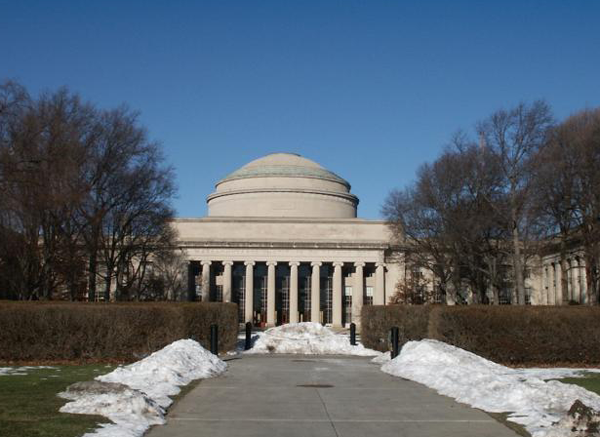
\includegraphics[width=0.9\columnwidth]{Figure1}
\caption{With Caption Below, be sure to have a good resolution image
(see item D within the preparation instructions).}
\label{fig:figure1}
\end{figure}

\subsection{References and Citations}

Use a numbered list of references at the end of the article, ordered
alphabetically by first author, and referenced by numbers in brackets
\cite{ethics,
Klemmer:2002:WSC:503376.503378,
Mather:2000:MUT,
Zellweger:2001:FAO:504216.504224}. For
papers from conference proceedings, include the title of the paper and
an abbreviated name of the conference (e.g., for Interact 2003
proceedings, use \textit{Proc. Interact 2003}). Do not include the
location of the conference or the exact date; do include the page
numbers if available. See the examples of citations at the end of this
document. Within this template file, use the \texttt{References} style
for the text of your citation.

Your references should be published materials accessible to the
public. Internal technical reports may be cited only if they are
easily accessible (i.e., you provide the address for obtaining the
report within your citation) and may be obtained by any reader for a
nominal fee. Proprietary information may not be cited. Private
communications should be acknowledged in the main text, not referenced
(e.g., ``[Robertson, personal communication]'').

\begin{table}
\centering
\begin{tabular}{|c|c|c|}
\hline
\tabhead{Objects} &
\multicolumn{1}{|p{0.3\columnwidth}|}{\centering\tabhead{Caption --- pre-2002}} &
\multicolumn{1}{|p{0.4\columnwidth}|}{\centering\tabhead{Caption --- 2003 and afterwards}} \\
\hline
Tables & Above & Below \\
\hline
Figures & Below & Below \\
\hline
\end{tabular}
\caption{Table captions should be placed below the table.}
\label{tab:table1}
\end{table}

\section{Sections}

The heading of a section should be in Helvetica 9-point bold, all in
capitals. Use Arial if Helvetica is not available. Sections should
not be numbered.

\subsection{Subsections}

Headings of subsections should be in Helvetica 9-point bold with
initial letters capitalized. For
sub-sections and sub-subsections, a word like \emph{the} or \emph{of}
is not capitalized unless it is the first word of the heading.)

\subsubsection{Sub-subsections}

Headings for sub-subsections should be in Helvetica 9-point italic
with initial letters capitalized. Standard {\textbackslash}section,
{\textbackslash}subsection, and {\textbackslash}subsubsection commands
will work fine.

\section{Figures/Captions}

Place figures and tables at the top or bottom of the appropriate
column or columns, on the same page as the relevant text
(see Figure~\ref{fig:figure1}). A figure or table may extend across both
columns to a maximum width of 17.78 cm (7 in.).

Captions should be Times New Roman 9-point bold. They should be numbered (e.g.,
``Table~\ref{tab:table1}'' or ``Figure~\ref{fig:figure1}''), centered
and placed beneath the figure or table. Please note that the words
``Figure'' and ``Table'' should be spelled out (e.g., ``Figure''
rather than ``Fig.'') wherever they occur.

Papers and notes may use color figures, which are included in the page
limit; the figures must be usable when printed in black and white in
the proceedings. The paper may be accompanied by a short video figure
up to five minutes in length. However, the paper should stand on its
own without the video figure, as the video may not be available to
everyone who reads the paper.

\section{Language, Style and Content}

The written and spoken language of SIGCHI is English. Spelling and
punctuation may use any dialect of English (e.g., British, Canadian,
US, etc.) provided this is done consistently. Hyphenation is
optional. To ensure suitability for an international audience, please
pay attention to the following:

\begin{itemize}
\item Write in a straightforward style.
\item Try to avoid long or complex sentence structures.
\item Briefly define or explain all technical terms that may be
unfamiliar to readers.
\item Explain all acronyms the first time they are used in your text---e.g.,
``Digital Signal Processing (DSP)''.
\item Explain local references (e.g., not everyone knows all city
names in a particular country).
\item Explain ``insider'' comments. Ensure that your whole audience
understands any reference whose meaning you do not describe (e.g.,
do not assume that everyone has used a Macintosh or a particular
application).
\item Explain colloquial language and puns. Understanding phrases like
``red herring'' may require a local knowledge of English. Humor and
irony are difficult to translate.
\item Use unambiguous forms for culturally localized concepts, such as
times, dates, currencies and numbers (e.g., ``1-5-97'' or ``5/1/97''
may mean 5 January or 1 May, and ``seven o'clock'' may mean 7:00 am or
19:00). For currencies, indicate equivalences---e.g., ``Participants
were paid 10,000 lire, or roughly \$5.''
\item Be careful with the use of gender-specific pronouns (he, she)
and other gendered words (chairman, manpower, man-months). Use
inclusive language that is gender-neutral (e.g., she or he, they,
s/he, chair, staff, staff-hours,
person-years). See~\cite{Schwartz:1995:GBF} for further advice and
examples regarding gender and other personal attributes.
\item If possible, use the full (extended) alphabetic character set
for names of persons, institutions, and places (e.g.,
Gr{\o}nb{\ae}k, Lafreni\'ere, S\'anchez, Universit{\"a}t,
Wei{\ss}enbach, Z{\"u}llighoven, \r{A}rhus, etc.). These characters
are already included in most versions of Times, Helvetica, and Arial
fonts.
\end{itemize}

\section{Accessibility}
The Executive Council of SIGCHI has committed to making SIGCHI conferences more inclusive for researchers, practitioners, and educators with disabilities. As a part of this goal, the all authors are asked to work on improving the accessibility of their submissions. Specifically, we encourage authors to carry out the following five steps:
\begin{enumerate}
        \item Add alternative text to all figures
        \item Mark table headings
        \item Add tags to the PDF
        \item Verify the default language
        \item Set the tab order to ``Use Document Structure''
\end{enumerate}
Unfortunately good tools do not yet exist to create tagged PDF files from Latex. LaTeX users will need to carry out all of the above steps in the PDF directly using Adobe Acrobat, after the PDF has been generated.
For more information and links to instructions and resources, please see:
{\url{http://chi2014.acm.org/authors/guide-to-an-accessible-submission}}.

\section{Page Numbering, Headers and Footers}

Please submit your anonymous version for reviewing with page numbers
centered in the footer. These must be removed in the final version of
accepted papers, as page numbers, headers, and footers will be added
by the conference printers. Comment out the {\textbackslash}pagenumbering
command at the top of the document to remove page numbers.




Scraps 
This exacerbates the need for tools and techniques that allow students in these large groups to approach the educational outcomes of one-on-one tutoring. It also opens up the possibility of

 Professors who repeatedly teach the same large engineering course have the luxury of seeing hundreds of students struggle with, and then complete, the same or similar assignments year after year. Like experienced doctors making their rounds through the computer lab, these professors have seen many of the designs and bugs before, and amaze students with their ability to see the problem, and the solution, right away. The steadily changing pool of teaching assistants have a fraction of that experience. Students are often waiting for help from the central repository of knowledge, the professor, who has limited time and attention, and the teaching assistants, who are more plentiful but less omniscient. And yet the students themselves are each becoming experts on their own bugs and designs.

Teachers' fears that students may just give each other answers  Their hints for other students may be comparable in quality to teachers' explanations if they genuinely want to help a fellow student, but are reluctant to just give away the knowledge they earned themselves through hard work.

PALS aims to create a reflective assessment process by combining two classical educational psychology frameworks: experiential learning (Kolb 1984) and collaborative learning (Piaget 1963, Vygotsky 1978).

Cognitive Tutor Author Tools (Opening the door to non-programmers) let teachers predict frequent correct and incorrect paths to a solution, and then annotate them with hints and feedback for students. Rather than ask teachers to predict students' behavior, Barnes et al. ran Markov decision processes (MDPs) on historical data of students' logic proof attempts, in order to algorithmically predict where hints are needed most. The hints themselves were still provided by instructors. 

It has been deployed within lectures in many different disciplines, including Physics (Mazur), Computer Science (Beth Simon), and Engineering (Nicol and Boyle). 

\subsection{Learner-Sourcing}
Summarize Juho's work.

We automatically presented students with these graphically rendered design alternatives that were better or worse than their own. 

Both website usage statistics and anecdotal evidence, including a student's unprompted class forum thank you note, suggest that a subset of students find the website to be very helpful. 

\section{Future Work}

While these systems 

\begin{itemize}
\item deploy 'real' version of Dear Beta system for 6.004x, which does double-duty for optimization as well, since that involves bugs too
\item do git diffs on optimization of betas this term to see what folks actually did this term?
\item create separate interface in which students can see their own place in space and time, along with diffs, and the ability to comment what they did (via API), with pull-down suggestions from other folks <-- more of a personal help system that motivates them to annotate.
\end{itemize}
How best do we close this loop, so that students benefit from the design alternatives and advice generated by classmates?


Teaching assistants are still more plentiful but less knowledgeable.

[a][width=0.65\paperwidth]
[b]Unfortunately, the effort of acquiring these statistics about the Beta was not trivial, and therefore very few students submitted their data to support this feature.
[c]thrown away: 

This system will need to be revised before redeployment. 

We hope to revise this system, based on insights about why it failed and why the system in the next section was successful.  the success of the system described in the next section. However, students were able to generate high quality optimization hints for another, simpler assignment, which is described in the next section. This gives us hope that, given the right structure and constraints, students will ultimately be able to both contribute constructively to and take advantage of a crowd-powered system full of helpful processor optimization hints. %system that can provide high quality hints to each student who optimizes their processor. % learner-source processor optimization as well. %We hope to take this feedback and redesign the tool so it can better support students through the optimization process.
[d]Students composed their Full Adders out of logic gates, e.g., NOR, NAND, and NOT. Each logic gate is composed of a particular number and arrangement of transistors.
[e]In other words, we did not empirically find any morphological differences between correct solutions with the same number of transistors. %This distribution is shown in Figure \ref{fig:figure1}.
[f]First comparison: student's design vs.: If student's FET count > expected FET count (expect == 2 xors, 3 NAND2s, 1 NAND3), compare against expected else compare against randomly chosen design with a larger number of FETs

Second comparison: student's design vs. best (best = 2 XOR, 3 NAND2).  If student has the best design they aren't asked for a second comparison.
